\section{Project Timeline and Contributions}
\label{sec:contributions}
The project was carried out by Chitraksh (CS23B054), Sudhanva (CS23B051) and
Rishikesh (CS23B015), under the guidance of Dr Vishnu Chalavadi.
Six experimental phases are complete. The current phase explores
RAMiT + YOLOv12 edge deployment.

\noindent\begin{minipage}{\linewidth}
\centering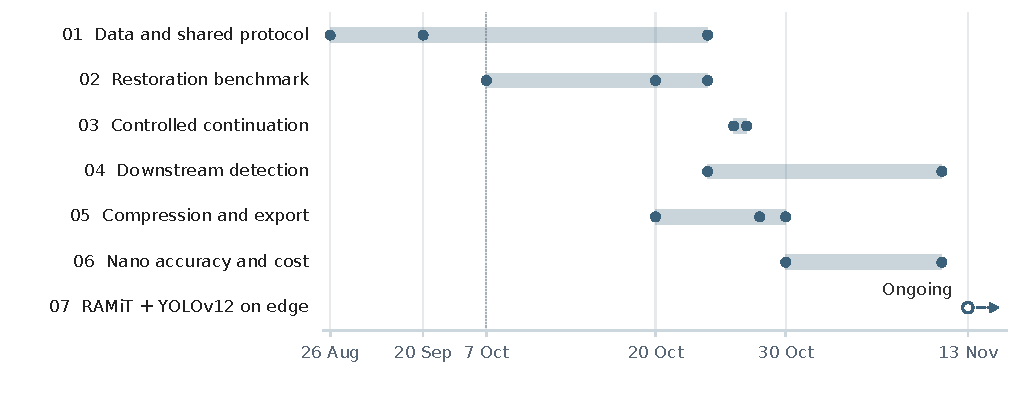
\includegraphics[width=\linewidth]{figures/work_timeline.pdf}
\captionof{figure}{Project timeline from dated records. Bars join the first and last milestones; dots identify records, not continuous daily effort. The axis is condensed before 7 October. Phase 7 is ongoing as of 13 November, with no completion date assigned.}
\label{fig:timeline}
\end{minipage}

\medskip
\noindent\begin{minipage}{\linewidth}
\captionof{table}{Individual and shared contributions to the six completed experimental phases. Entries identify recorded work; they do not assign exclusive ownership or percentages of effort.}
\label{tab:work-allocation}
\small\renewcommand{\arraystretch}{1.15}
\begin{tabularx}{\linewidth}{@{}p{.18\linewidth}YYY@{}}\toprule
Work package & Chitraksh & Sudhanva & Rishikesh\\\midrule
Data and protocol & Source/split review; metric interpretation & Split tooling; training configuration & Weather-level evaluation\\\addlinespace[3pt]
Six-model benchmark & Result review; benchmark context & Model implementation; training and selection & Cross-weather evaluation\\\addlinespace[3pt]
Continuation & Joint result review & Eight matched arms; validation selection & Joint result review\\\addlinespace[3pt]
Detection & Joint result review & Pilot tooling; resolution controls & Raw/resize/restored analysis\\\addlinespace[3pt]
Compression/export & Custom quantizer; pruning tooling & Trained export; adapter and checks & Compression/export evaluation\\\addlinespace[3pt]
Nano measurements & Joint result review & Nano runtime; export integration & Device-path analysis; FPS and power review\\\bottomrule
\end{tabularx}
\end{minipage}

\begin{multicols}{2}\raggedcolumns
\textbf{Research and compression.} Chitraksh's work connects source and
benchmark review to custom weight quantization and pruning. The integrated
edge handoff credits his quantizer; the 20 and 28 October commits record
these implementations. The tested weight grid was rejected by the numerical
screen.

\textbf{Models and integration.} Sudhanva configured and trained the models,
implemented the matched continuation experiments, and integrated the trained
exports and Nano runtime. Validation retained the original epoch-51 model.

\textbf{Evaluation.} Rishikesh's work covers restoration and detector
comparisons, export evaluation, and interpretation of Nano accuracy,
runtime and power. All three reviewed the experimental outputs and final
interpretation.

\textbf{Current work.} RAMiT + YOLOv12 integration and measured edge deployment
remain ongoing. No end-to-end accuracy or throughput result is yet claimed
for that combination.
\end{multicols}
\clearpage
